\documentclass[a4paper,12pt]{article}
\author{}
\date{}
\usepackage[papersize={216mm,330mm},tmargin=20mm,bmargin=20mm,lmargin=20mm,rmargin=20mm]{geometry}
\usepackage[english]{babel}
\usepackage[utf8]{inputenc}
\usepackage{amsmath,amssymb,mathabx}%\for eqref
\usepackage{lscape}
\usepackage{graphicx}
\usepackage[colorinlistoftodos]{todonotes}
\usepackage{fancyhdr}
 
\pagestyle{fancy}
\fancyhf{}
\lhead{Universidad de San Andrés}
\chead{\thepage}
\rhead{Departamento de Economía}
\lfoot{Big Data}
\cfoot{TP2}
\rfoot{Servent, Musich \& Cuellar}

\title{\Large \textbf{Universidad de San Andrés}\\ Departamento de Economía \\ Big Data \\ \vspace{5mm} \LARGE \textbf{Trabajo Práctico Nº 2}  \vspace{0cm} \normalsize 
  \vspace{0cm} \Large \textit{}}

\begin{document}
\maketitle

\section*{Ejercicios}
\begin{enumerate}
\item El documento elaborado por el INDEC detalla con profundidad la metodología adoptada para medir la pobreza y la indigencia en Argentina. Central en este enfoque es el método de medición indirecta, que se basa en establecer "líneas" o umbrales de ingresos. La "Línea de Indigencia" (LI) se configura para identificar si los ingresos de un hogar son suficientes para cubrir una Canasta Básica Alimentaria (CBA). Esta canasta está diseñada para satisfacer un umbral mínimo de necesidades energéticas y proteicas, reflejando el patrón de consumo de alimentos de la población de referencia.

Por otro lado, la "Línea de Pobreza" (LP) tiene un alcance más amplio. Va más allá de las necesidades alimentarias y considera otros consumos esenciales no alimentarios. Así, se forma la Canasta Básica Total (CBT), que incluye aspectos como vestimenta, transporte, educación, salud, entre otros. Esta canasta se compara con los ingresos de los hogares, información que se extrae de la Encuesta Permanente de Hogares (EPH).

Es crucial entender que la Canasta Básica Alimentaria ha sido determinada basándose en diferentes Encuestas de Ingresos y Gastos a lo largo del tiempo. Estas encuestas han mostrado cambios en los hábitos de consumo de la población argentina. Por ejemplo, en años recientes, se ha observado una reducción en el gasto alimentario y un incremento en otros rubros, como el transporte y la vivienda. Estas variaciones tienen un impacto directo en cómo se mide la pobreza, ya que afectan la distancia entre la Línea de Indigencia y la Línea de Pobreza. Por ello, el INDEC subraya la importancia de realizar actualizaciones metodológicas periódicas y considerar una variedad de factores para garantizar una medición precisa y representativa de la pobreza en el país.  \normalsize  
\item 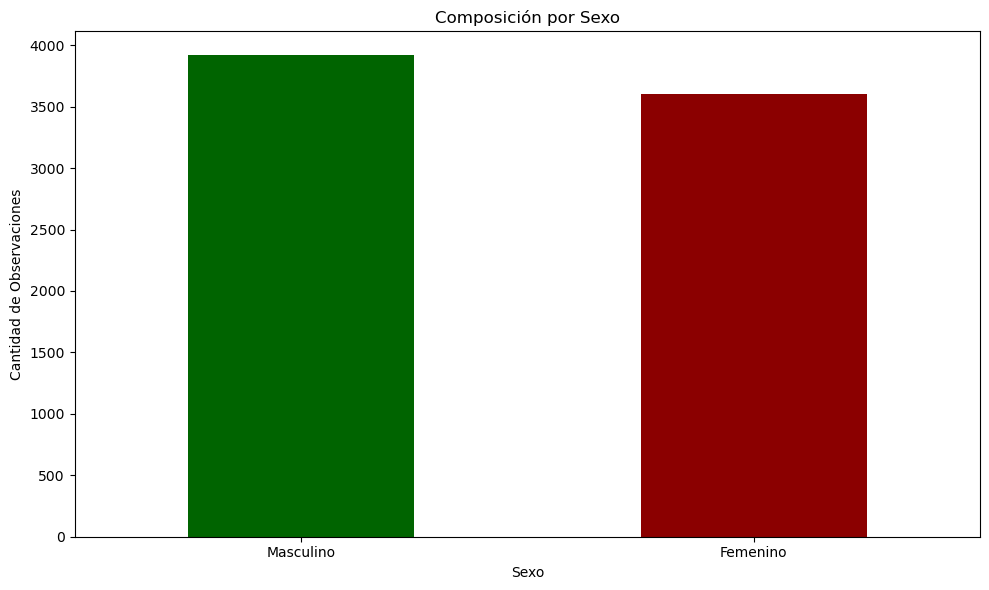
\includegraphics[width=1.0\linewidth]{compo.png}
 \normalsize 
\item 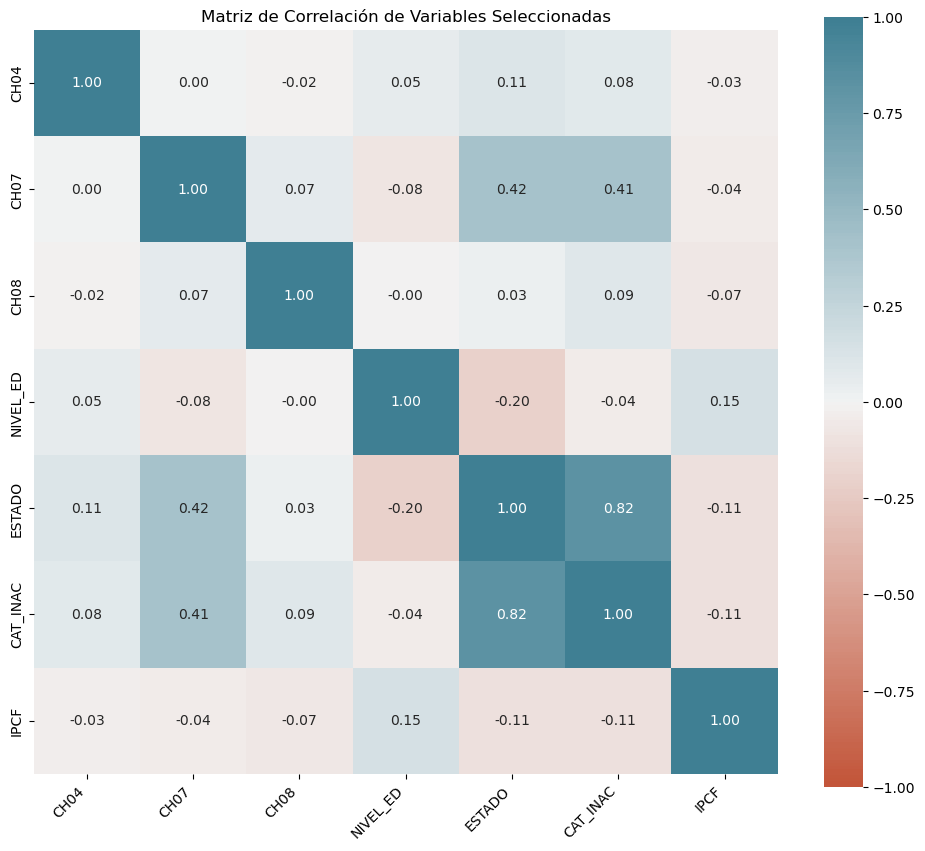
\includegraphics[width=1.0\linewidth]{matriz.png} \normalsize 
 \normalsize

\end{enumerate}

\end{document}